\glsresetall

% \section{Abstract}


Microbiome data are sparse and high-dimensional, so effective visualization of these data requires dimensionality reduction. To date, the most commonly used method for dimensionality reduction in the microbiome is calculation of between-sample microbial differences (beta diversity), followed by Principal Coordinates Analysis (PCoA). Uniform Manifold Approximation and Projection (UMAP) is an alternative method that can reduce the dimensionality of beta diversity distance matrices. Here, we demonstrate the benefits and limitations of using UMAP for dimensionality reduction on microbiome data. Using real data, we demonstrate that UMAP can improve the representation of clusters, especially when the clusters are composed of multiple subgroups. Additionally, we show that UMAP provides improved correlation of biological variation along a gradient with a reduced number of coordinates of the resulting embedding. Finally, we provide parameter recommendations that emphasize the preservation of global geometry. We therefore conclude that UMAP should be routinely used as a complementary visualization method for microbiome beta diversity studies.


\section{Importance}
UMAP provides an additional method to visualize microbiome data. The method is extensible to any beta diversity metric used with PCoA, and our results demonstrate that UMAP can indeed improve visualization quality and correspondence with biological and technical variables of interest. The software to perform this analysis is available under an open-source license and can be obtained at https://github.com/knightlab-analyses/umap-microbiome-benchmarking; additionally, we have provided a QIIME 2 plugin for UMAP at\\ https://github.com/biocore/q2-umap.

\section{Observation}
An important step in microbiome research is visualizing the relationships between samples. In the study of microbial communities through next generation sequencing (NGS), these comparisons are typically done through the visualization of beta diversities with principal coordinates analysis (PCoA) \cite{Kruskal1978-xx} (Figure~\ref{umap_figS1}). Although alternatives such as conventional principal component analysis (PCA), non-metric multidimensional scaling  (NMDS) \cite{Kruskal1964-dn} and t-distributed stochastic neighbor embedding (t-SNE) \cite{Van_der_Maaten2008-af} are sometimes applied, PCoA in particular has been widely adopted by the microbiome community.  Due to the high dimensional and highly sparse nature of the data, which presents challenges on sequence count data \cite{Aitchison1983-mz,Martino2019-op}, one major benefit of PCoA over other methods on untransformed count data is that it accommodates a generalized distance matrix (of beta diversities, for the microbiome).  This allows use of distance metrics that are better-suited for sparse data (e.g., Bray-Curtis \cite{Bray1957-fg}, Jaccard \cite{Jaccard1912-bk}, UniFrac \cite{Lozupone2005-aj}).
Uniform Manifold Approximation and Projection (UMAP) \cite{McInnes2018-zd}  is a method that has gained traction in single-cell genomics analysis \cite{Hao2020-gu}. Whereas PCoA performs an eigendecomposition that focuses on linearly preserving the pairwise distances between the samples (global structure), UMAP uses a non-linear graph construction and embedding method to optimize an objective that allows for a trade-off between emphasizing local structures and preserving distances globally. This trade-off is primarily controlled by the `n\_neighbors' and `min\_dist' parameters of UMAP. The `n\_neighbors' parameter controls the number of neighbors whose local topology is preserved, so global distances are preserved when it is high. The `min\_dist' parameter controls the minimum distance between samples in the embedding, which affects the spread of clusters. Low values of `min\_dist' allow UMAP to emphasize the similarity of dense clusters of samples, whereas larger values of `min\_dist' will focus on preserving distances more broadly.
Both UMAP and PCoA operate on a generalized distance (beta diversity) matrix, appropriate for microbiome data (Figure~\ref{umap_figS1}). While the use of UMAP on microbiome data has been noted (11) the utility of UMAP on microbiome data remains underexplored. Using real datasets, we compared both visual qualities and quantitative measures of UMAP to PCoA on well understood datasets. We additionally applied UMAP to data from the Human Microbiome Project (HMP) \cite{The_Human_Microbiome_Project_Consortium2012-og} to demonstrate its characteristics on a larger dataset with more complex sources of variation.
Discrete clusters are one common pattern that microbial communities can exhibit \cite{Kuczynski2010-gu}. The `keyboard data' from \cite{Fierer2010-dp} contains 16S samples (n = 99, features  = 1399, 5\% dense) from the keyboards and fingers of 3 subjects. PCoA on the Aitchison distances on these samples can recover the cluster structure of the subjects in the data (Figure~\ref{umap_fig1}A). We compared this to UMAP (n\_neighbors = 15 and n\_neighbors = 80, min\_dist = 1) and found that UMAP can also recover the cluster structure of the subjects (Figure~\ref{umap_fig1} B,C). We also saw that UMAP produced two-dimensional coordinates with improved separation within subjects by sample type. This was further supported by improved LDA classification of sample type stratified by subject (Table~\ref{umap_table1}).


\begin{figure}[htbp]
\centering
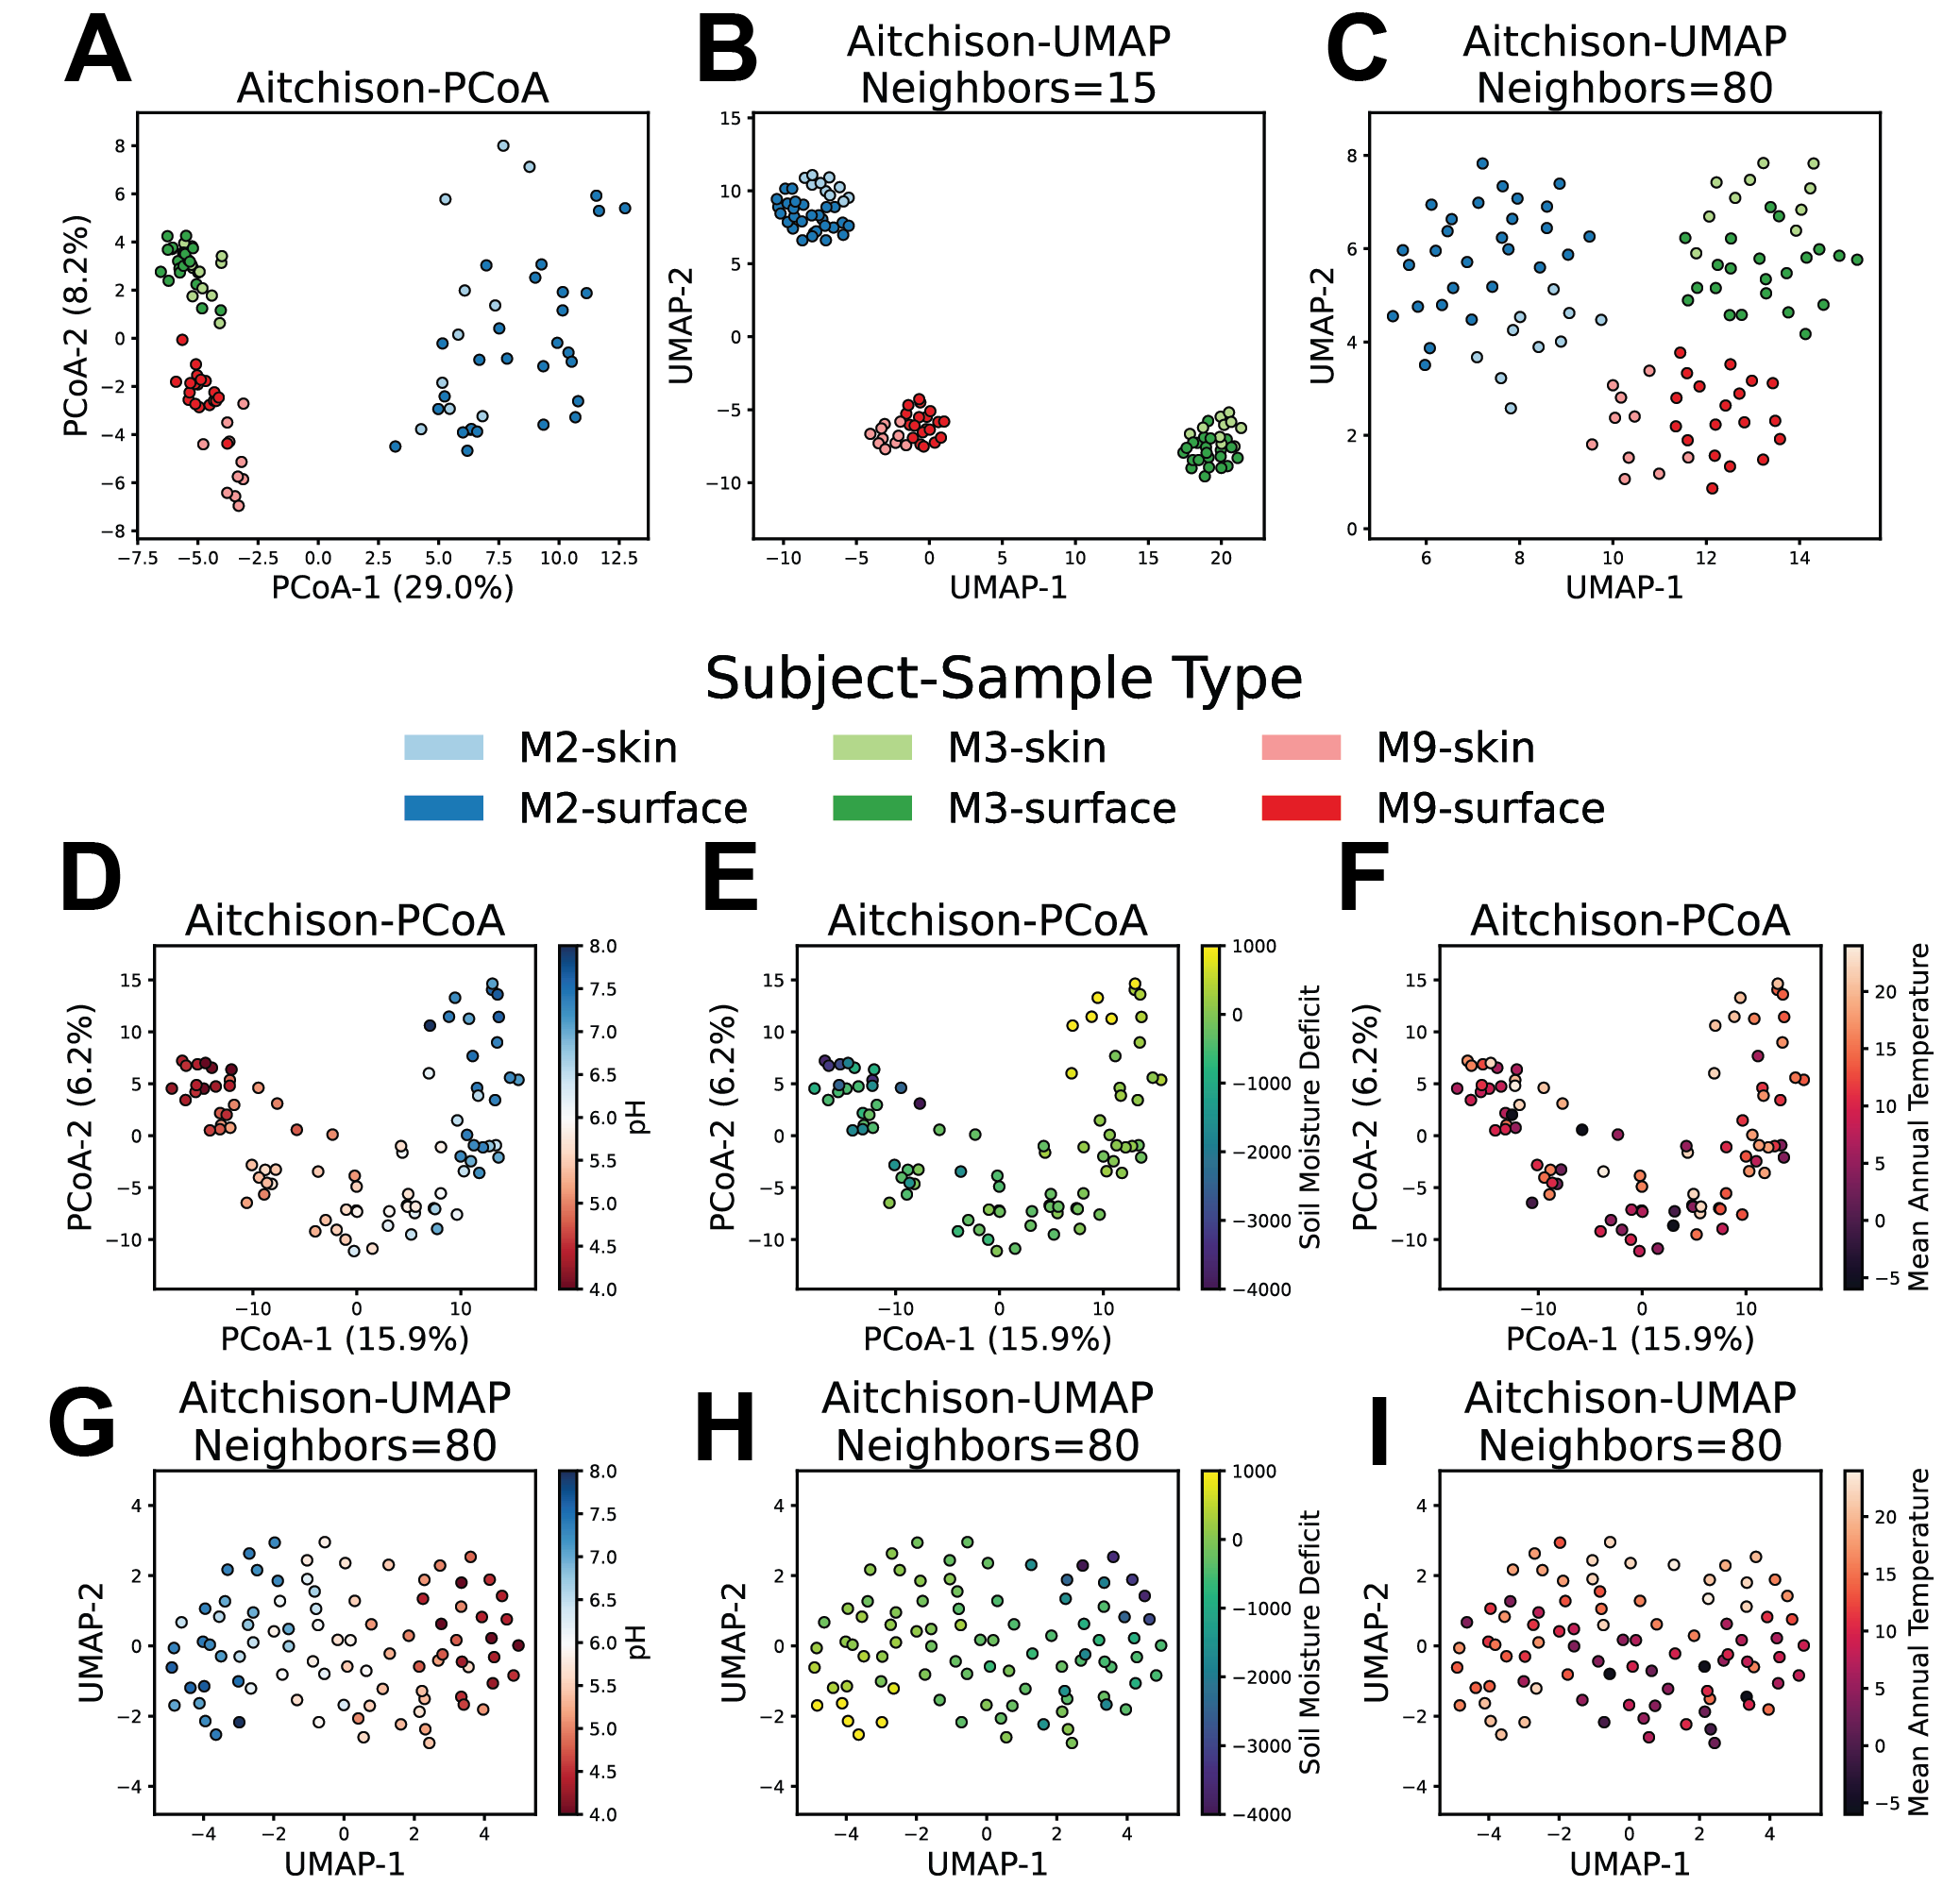
\includegraphics[width=0.8\textwidth]{umap-figures/figure01.png}
\caption[Comparison of PCoA and UMAP visualizations of cluster and gradient patterns on real data.]{\textbf{ Comparison of PCoA and UMAP visualizations of cluster and gradient patterns on real data. } The keyboard data set contains samples from three different subjects’ keyboards (surface) and their hands (skin). (A) PCoA on Aitchison distances (pseudocount = 1) demonstrates a strong separation between M2 and the other subjects, as well as separation between subjects M3 and M9. (B) A UMAP (n\_neighbors = 15, min\_dist = 1) visualization demonstrates stronger clustering by subject, with a different relative positioning of the clusters by subject. The plot also emphasizes clustering by sample type. (C) UMAP with an increased n\_neighbors parameter (n\_neighbors = 80, min\_dist = 1) reflects the same relative positioning of clusters as PCoA. It also demonstrates the improved localization by sample type within subjects. (D) On the “88 soils” data, PCoA on the Aitchison distances demonstrates a horseshoe pattern with pH distributed along the horseshoe. (E) Soil moisture deficit is also distributed along the horseshoe, and (F) there is not a strong association between mean annual temperature and position on the PCoA. (G) In the UMAP (n\_neighbors = 80, min\_dist = 1), followed by centering/rotation with PCA }
\label{umap_fig1}
\end{figure}

\begin{sidewaystable}[]
\caption{Linear Discriminant Analysis on Aitchison Embedding 10 different initializations for UMAP}
\singlespace
\label{umap_table1}
\centering
\begin{tabular}{llllllll} \hline
\multicolumn{1}{c}{} & \multicolumn{1}{c}{Metric} & \multicolumn{1}{c}{\begin{tabular}[c]{@{}c@{}}PCoA \\ Dims=2\end{tabular}} & \multicolumn{1}{c}{\begin{tabular}[c]{@{}c@{}}PCoA\\ Dims=3\end{tabular}} & \multicolumn{1}{c}{\begin{tabular}[c]{@{}c@{}}UMAP\\ Neighbors=15 \\ Dims=2\end{tabular}} & \multicolumn{1}{c}{\begin{tabular}[c]{@{}c@{}}UMAP\\ Neighbors=80 \\ Dims=2\end{tabular}} & \multicolumn{1}{c}{\begin{tabular}[c]{@{}c@{}}UMAP\\ Neighbors=98\\ Dims=2\end{tabular}} & \multicolumn{1}{c}{\begin{tabular}[c]{@{}c@{}}UMAP\\ Neighbors=98\\ Dims=2\end{tabular}} \\ \hline
\multirow{2}{*}{host} & \begin{tabular}[c]{@{}l@{}}mean\\ (Accuracy)\end{tabular} & 0.990 & 1.000 & 1.000 & 1.000 & 1.000 & 1.000 \\
 & std &  &  & 0.000 & 0.000 & 0.000 & 0.000 \\ \hline
\multirow{2}{*}{M2-type} & \begin{tabular}[c]{@{}l@{}}mean\\ (Accuracy)\end{tabular} & 0.789 & 0.921 & 0.974 & 0.992 & 0.989 & 0.997 \\
 & std &  &  & 0.012 & 0.013 & 0.014 & 0.008 \\ \hline
\multirow{2}{*}{M3-type} & \begin{tabular}[c]{@{}l@{}}mean\\ (Accuracy)\end{tabular} & 0.781 & 0.844 & 0.856 & 0.831 & 0.828 & 0.900 \\
 & std &  &  & 0.049 & 0.059 & 0.065 & 0.041 \\ \hline
\multirow{2}{*}{M9-type} & \begin{tabular}[c]{@{}l@{}}mean\\ (Accuracy)\end{tabular} & 0.931 & 0.966 & 0.990 & 0.969 & 0.972 & 0.976 \\
 & std &  &  & 0.017 & 0.025 & 0.027 & 0.023 \\ \hline
\multirow{2}{*}{host} & \begin{tabular}[c]{@{}l@{}}mean\\ (Silhouette)\end{tabular} & 0.647 & 0.601 & 0.794 & 0.548 & 0.533 & 0.500 \\
 & std &  &  & 0.069 & 0.011 & 0.018 & 0.008 \\ \hline
\multirow{2}{*}{M2-type} & \begin{tabular}[c]{@{}l@{}}mean\\ (Silhouette)\end{tabular} & 0.095 & 0.127 & 0.297 & 0.306 & 0.304 & 0.263 \\
 & std &  &  & 0.019 & 0.012 & 0.012 & 0.008 \\ \hline
\multirow{2}{*}{M3-type} & \begin{tabular}[c]{@{}l@{}}mean\\ (Silhouette)\end{tabular} & 0.181 & 0.288 & 0.231 & 0.181 & 0.184 & 0.175 \\
 & std &  &  & 0.036 & 0.065 & 0.066 & 0.026 \\ \hline
\multirow{2}{*}{M9-type} & \begin{tabular}[c]{@{}l@{}}mean\\ (Silhouette)\end{tabular} & 0.534 & 0.441 & 0.449 & 0.383 & 0.385 & 0.308 \\
 & std &  &  & 0.023 & 0.013 & 0.029 & 0.020 \\ \hline
\end{tabular}
\end{sidewaystable}

To quantitatively assess the dimensionality reduction, we performed a supervised classification with Linear Discriminant Analysis (LDA) and as well as an unsupervised evaluation of clustering using the silhouette measure on the low dimensional representations. The LDA classification, which solely measures separability, demonstrated higher accuracy of sample type (stratified by subject) on UMAP with two components compared to PCoA with two or three components for all subjects (Table~\ref{umap_table1}). Silhouette scores, which measure cluster separation and density, demonstrated that host separation is improved with UMAP with a low `n\_neighbors' value, but not for a higher `n\_neighbors' value, which is likely due to the reduced distance between clusters in the UMAP coordinates with higher `n\_neighbors'. The method with the highest within-host sample-type silhouette varied for each host. A simulated missing data analysis, where entries were randomly masked from samples, demonstrated that these results are sensitive to missing values (Figure~\ref{umap_figS2}).
In dimensionality reduction, it is not only important for clusters to be separated; the positioning of clusters with respect to their similarity to other clusters, i.e. preserving global distances, is desirable. In the PCoA visualization (Figure~\ref{umap_fig1}A) the samples of subjects M3 and M9 are similar to each other in the plot, and both are distant from M2. This corresponds with the expectation that M3 and M9 are more similar, because they shared an office. Additionally, this agrees with the original distances, where the mean Aitchison distance between M3 and M9 samples is $13.87 \pm 0.11$, (95\% CI), whereas the mean M2-M3 distance is $19.89 \pm 0.11$, (95\% CI), and the mean M2-M9 distance is $18.94 \pm 0.12$. (95\% CI). However, for UMAP with n\_neighbors = 15 in Figure~\ref{umap_fig1}B,  the relative position of the clusters has changed (M9 is closer to M2 than it is to M3). Using the default ‘spectral’ initialization option, which is recommended for preserving global structure \cite{Kobak2021-ih}, we found that on only 34 / 50  initializations with different random seeds and n\_neighbors = 15, UMAP produced clusters with the correct relative positioning. However, when we increase the parameter to n\_neighbors = 80, which represents a large majority of the samples, the visualization retains separation by subject (Figure~\ref{umap_fig1}C), and 50 / 50 initializations produced clusters with the correct relative positioning.

Ecological gradients are another common pattern that microbial communities can exhibit \cite{Kuczynski2010-gu}. The `88 soils' data from \cite{Lauber2009-jo} contains 16S samples (n = 88, features = 5627, 4\% dense) from 88 different soils with additional measurements of the soil. A Bio-Env test \cite{Clarke1993-ad} reveals that the top three soil variates corresponding with the Aitchison distances are pH, moisture deficit, and mean annual temperature (Table~\ref{umap_table2}). In the PCoA of the Aitchison distances, which displays a horseshoe artifact \cite{Morton2017-bs,Diaconis2008-ah}, pH is distributed along the horseshoe (Fig 1d). To quantitatively assess the visualization of gradients in the data, similarly to \cite{Kuczynski2010-gu}, we calculated the Spearman correlation of the components of the ordination with the ecological variable. We found that soil pH is strongly correlated with the first component (Spearman r = 0.934) (Table~\ref{umap_table2}). Soil Moisture deficit is also distributed along the horseshoe (Figure~\ref{umap_fig1}E), with PCoA-1 (Spearman r = 0.828). There is a mild correlation between Mean Annual Temperature and the second PCoA coordinate (Spearman r = 0.313), although a pattern is difficult to see visually due to the horseshoe artifact (Figure~\ref{umap_fig1}F).

\begin{table}[]
\caption{BioEnv selected top 3 combinations of variables correlated with Aitchison Distances}
\label{umap_table2}
\centering
\begin{tabular}{lll} \hline
Variables & \# of variables & Correlation \\ \hline
ph & 1 & 0.649058 \\
annual\_season\_temp, ph & 2 & 0.609095 \\
annual\_season\_temp, ph, soil\_moisture\_deficit & 3 & 0.583832 \\ \hline
\end{tabular}
\end{table}

On the gradient problem, we fit UMAP with the parameters used with the keyboard data (min\_dist = 1, n\_neighbors = 80). Since the UMAP algorithm does not guarantee the direction with the most variance in its output coordinates is axis-aligned, we use PCA to identify the direction of maximum variance in the UMAP embedding and rotate the UMAP coordinates so that this direction is aligned with the x-axis. The visualization shows reduced horseshoe-like warping, in contrast to the PCoA (Figure~\ref{umap_fig1}G). Additionally, the pH gradient is highly correlated with the first principal component of the embedding (Spearman r = -0.931). Furthermore, the soil moisture deficit is displayed clearly across the diagonal of the embedding (Figure~\ref{umap_fig1}H), and is correlated with both components of the axes (Table~\ref{umap_table3}). Finally, the mean annual temperature has a much clearer association in two-dimensional UMAP coordinates compared to the first two components of PCoA, with a higher Spearman correlation with the second component (r = 0.478 for n\_neighbors = 80, r = -0.604 for n\_neighbors = 87). PCoA exhibits maximum Spearman correlation with mean annual temperature in its third component (r = -0.567). So while a single axis of PCoA may be more correlated with the gradient, UMAP is able to display each of the gradients in fewer dimensions.

\begin{table}[]
\caption{Spearman Correlation of Environmental Variables with Embedding.}
\label{umap_table3}
\centering
\begin{tabular}{lllll} \hline
PC & method & category & spearmanr & p-value \\ \hline
1 & PCoA & annual\_season\_temp & 0.173 & 0.106514 \\
1 & UMAP Neighbors=80 & annual\_season\_temp & -0.184 & 0.085465 \\
1 & UMAP Neighbors=87 & annual\_season\_temp & 0.218 & 0.041722 \\
2 & PCoA & annual\_season\_temp & 0.313 & 0.002998 \\
2 & UMAP Neighbors=80 & annual\_season\_temp & 0.478 & 0.000002 \\
2 & UMAP Neighbors=87 & annual\_season\_temp & -0.604 & 0.000000 \\
3 & PCoA & annual\_season\_temp & -0.568 & 0.000000 \\
1 & PCoA & ph & 0.934 & 0.000000 \\
1 & UMAP Neighbors=80 & ph & -0.931 & 0.000000 \\
1 & UMAP Neighbors=87 & ph & 0.928 & 0.000000 \\
2 & PCoA & ph & 0.104 & 0.333014 \\
2 & UMAP Neighbors=80 & ph & -0.009 & 0.930266 \\
2 & UMAP Neighbors=87 & ph & 0.020 & 0.850003 \\
1 & PCoA & soil\_moisture\_deficit & 0.828 & 0.000000 \\
1 & UMAP Neighbors=80 & soil\_moisture\_deficit & -0.848 & 0.000000 \\
1 & UMAP Neighbors=87 & soil\_moisture\_deficit & 0.850 & 0.000000 \\
2 & PCoA & soil\_moisture\_deficit & -0.040 & 0.711593 \\
2 & UMAP Neighbors=80 & soil\_moisture\_deficit & -0.367 & 0.000436 \\
2 & UMAP Neighbors=87 & soil\_moisture\_deficit & 0.327 & 0.001882 \\ \hline
\end{tabular}
\end{table}

	Next, we compared PCoA and UMAP on data from the HMP(n = 8,280, features = 13,318, 0.08\% dense) \cite{The_Human_Microbiome_Project_Consortium2012-og}. These samples are from various body sites and individuals, with a large portion of samples processed with primers for two different variable regions of 16S. As noted in \cite{Debelius2016-ym}, the PCoA on unweighted UniFrac distances shows differences in primers are not visible in the first two coordinates (Figure~\ref{umap_fig2}A). Localization by body sites, however, is more apparent (Figure~\ref{umap_fig2}B). Clustering by primer is instead visible in the third component of the PCoA (Figure~\ref{umap_figS3}A), where clustering by body site is also apparent (Figure~\ref{umap_figS3}B). We also fit a two-dimensional UMAP (min\_dist = 1, n\_neighbors = 800) to the same data. UMAP is able to separate a majority of the samples by variable region (Figure~\ref{umap_fig2}C). It also produces more distinct clusters by body site.

\begin{figure}[htbp]
\centering
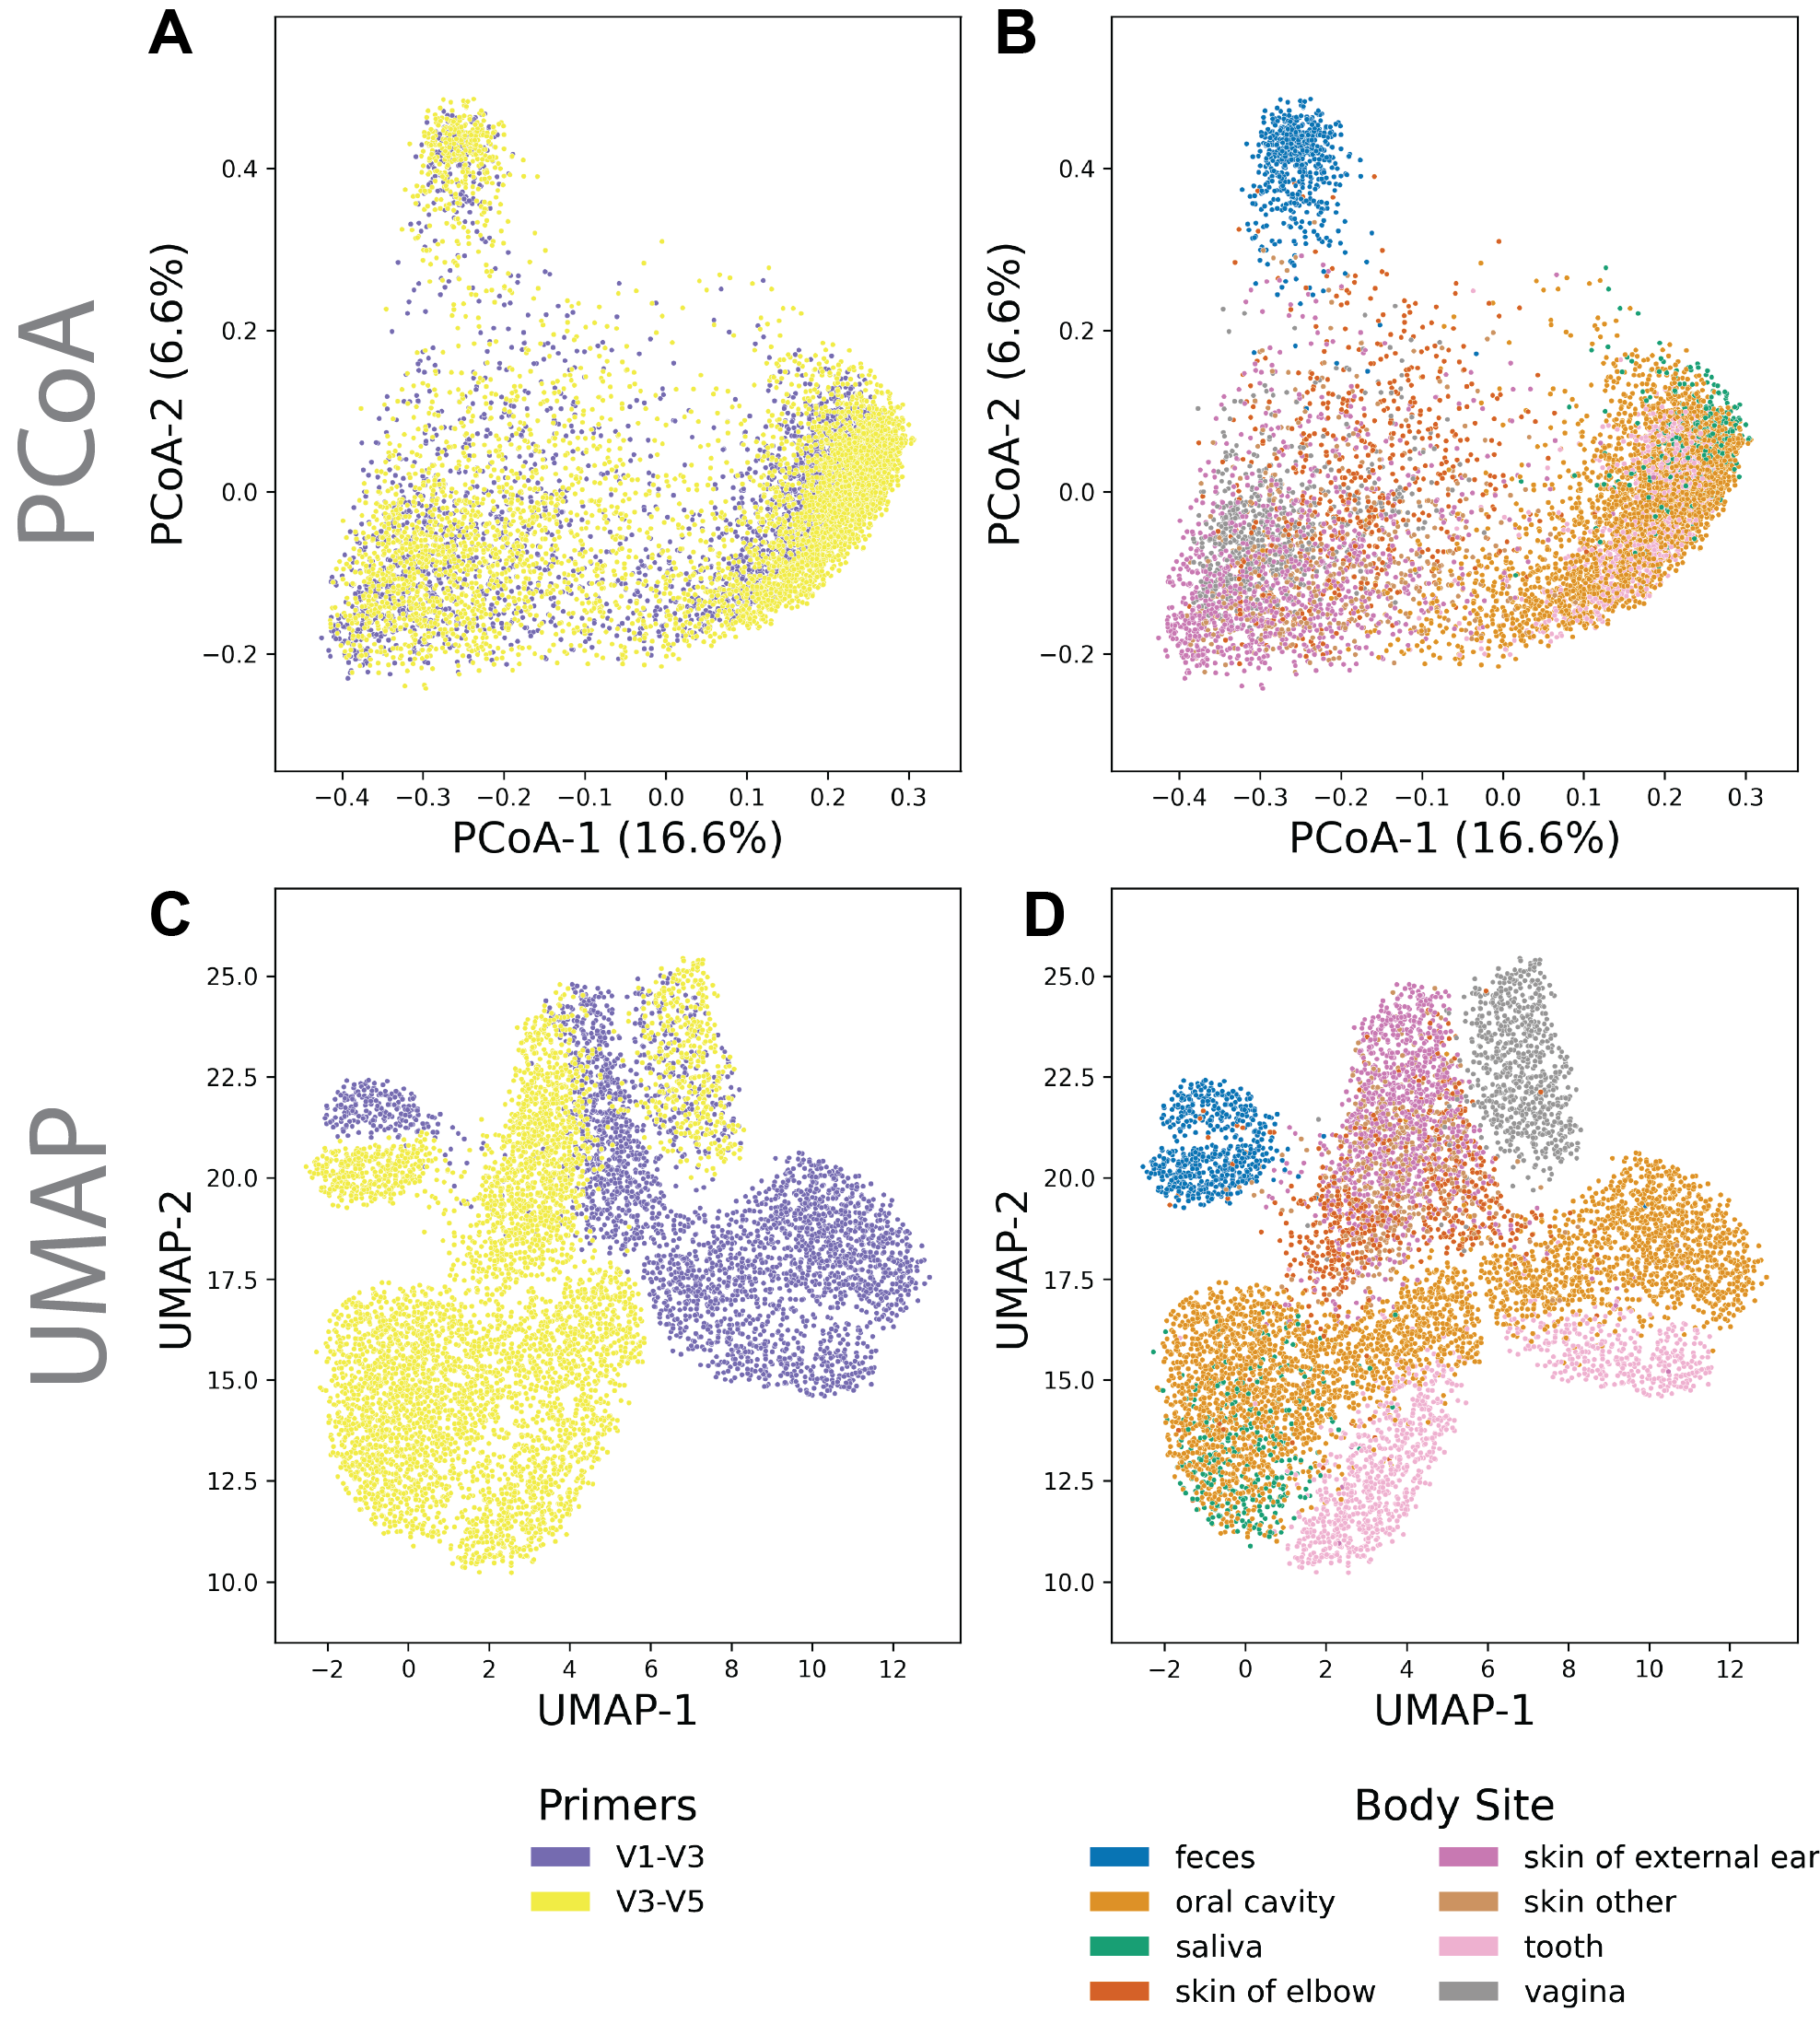
\includegraphics[width=\textwidth]{umap-figures/figure02.png}
\caption[PCoA and UMAP comparison on 8,280 samples from the Human Microbiome Project (HMP).]{\textbf{PCoA and UMAP comparison on 8,280 samples from the Human Microbiome Project (HMP).}  In the HMP data, when samples prepared with different primers are analyzed jointly, (A) there appears to be no separation between primers in the first two coordinates of PCoA and (B) mild separation by body site. In the same number of dimensions, UMAP is able to both (C) emphasize the differences between samples prepared with different variable regions and (D) improve clustering by body site. Both methods use the unweighted UniFrac distances on the HMP data rarefied to 1,000 sequences per sample.}
\label{umap_fig2}
\end{figure}

To quantify the clustering in the HMP data, we trained a k-Nearest Neighbors (kNN) classifier on the respective variables with 10-fold cross validation and reported the mean accuracy on the test folds. We trained kNN models on the first one, two, and three components of the PCoA, as well as fit UMAP embeddings for the respective number of dimensions. We found that kNN on a one-dimensional UMAP can outperform the sample site kNN for PCoA on up to 3 dimensions (Table~\ref{umap_table4}). kNN trained on a two-dimensional UMAP was able to distinguish primers more accurately than kNN on the first two principal coordinates. This indicates that UMAP is capable of representing multiple sources of variability in microbiome datasets with thousands of samples more distinctly and in fewer dimensions than PCoA.

\begin{table}[]
\caption{Comparison of 10-fold cross-validation accuracy of kNN in biological and technical variates}
\label{umap_table4}
\centering
\begin{tabular}{llll}
\hline \# of dimensions & Method & Target & Mean Accuracy \\ \hline
1 & PCoA & body\_habitat & 0.755556 \\
2 & PCoA & body\_habitat & 0.844203 \\
3 & PCoA & body\_habitat & 0.878140 \\
1 & UMAP Neighbors=8279 & body\_habitat & 0.924638 \\
1 & UMAP Neighbors=800 & body\_habitat & 0.929710 \\
2 & UMAP Neighbors=800 & body\_habitat & 0.932609 \\
2 & UMAP Neighbors=8279 & body\_habitat & 0.932850 \\
3 & UMAP Neighbors=800 & body\_habitat & 0.947222 \\
3 & UMAP Neighbors=8279 & body\_habitat & 0.947222 \\
1 & PCoA & qiita\_study\_id & 0.548913 \\
2 & PCoA & qiita\_study\_id & 0.570048 \\
1 & UMAP Neighbors=8279 & qiita\_study\_id & 0.805435 \\
1 & UMAP Neighbors=800 & qiita\_study\_id & 0.808937 \\
2 & UMAP Neighbors=8279 & qiita\_study\_id & 0.860990 \\
3 & PCoA & qiita\_study\_id & 0.891304 \\
2 & UMAP Neighbors=800 & qiita\_study\_id & 0.895773 \\
3 & UMAP Neighbors=800 & qiita\_study\_id & 0.916184 \\
3 & UMAP Neighbors=8279 & qiita\_study\_id & 0.916184 \\ \hline
\end{tabular}
\end{table}

	Finally, we explored a general-purpose recommendation for parameters. The parameters in this study were chosen to emphasize preserving the global structure of the data, by setting the `min\_dist' to its maximum of 1, increasing `n\_neighbors' from its default, and using default values for the rest of the parameters. In accordance with this goal, we set `n\_neighbors' to its maximum (n - 1 in general, 98 for soils, 87 for keyboard, and 8279 for the HMP) and re-ran the previous analyses. With this parameter setting, the results remain largely unchanged (Table~\ref{umap_table4}).
	Our benchmarks demonstrate the potential for improved performance and interpretability for both cluster and gradient microbiome data by using UMAP with its parameters set with the intent to preserve global geometry. Given that both algorithms provide different guarantees with respect to the preservation of distances in embeddings, we conclude that UMAP should be routinely used for microbiome analyses as a complement to PCoA. In order to facilitate using UMAP, we have made it conveniently available via QIIME2 \cite{Bolyen2019-fq} and Qiita \cite{Gonzalez2018-ez} plugins.
	
	
\section{Acknowledgements}

This work was supported in part by IBM Research AI through the AI Horizons Network, the Center for Microbiome Innovation at UC San Diego.

Chapter~\ref{chapter_umap}, in full, is a reprint of the material as it appears in ``Uniform Manifold Approximation and Projection (UMAP) Reveals Composite Patterns and Resolves Visualization Artifacts in Microbiome Data.'' George Armstrong, Cameron Martino, Gibraan Rahman, Antonio Gonzalez, Yoshiki Vázquez-Baeza, Gal Mishne, and Rob Knight.  \textit{mSystems 6}, 2021. The dissertation author was the primary investigator and the first author of this paper.
